\documentclass[1p]{elsarticle_modified}
%\bibliographystyle{elsarticle-num}

%\usepackage[colorlinks]{hyperref}
%\usepackage{abbrmath_seonhwa} %\Abb, \Ascr, \Acal ,\Abf, \Afrak
\usepackage{amsfonts}
\usepackage{amssymb}
\usepackage{amsmath}
\usepackage{amsthm}
\usepackage{scalefnt}
\usepackage{amsbsy}
\usepackage{kotex}
\usepackage{caption}
\usepackage{subfig}
\usepackage{color}
\usepackage{graphicx}
\usepackage{xcolor} %% white, black, red, green, blue, cyan, magenta, yellow
\usepackage{float}
\usepackage{setspace}
\usepackage{hyperref}

\usepackage{tikz}
\usetikzlibrary{arrows}

\usepackage{multirow}
\usepackage{array} % fixed length table
\usepackage{hhline}

%%%%%%%%%%%%%%%%%%%%%
\makeatletter
\renewcommand*\env@matrix[1][\arraystretch]{%
	\edef\arraystretch{#1}%
	\hskip -\arraycolsep
	\let\@ifnextchar\new@ifnextchar
	\array{*\c@MaxMatrixCols c}}
\makeatother %https://tex.stackexchange.com/questions/14071/how-can-i-increase-the-line-spacing-in-a-matrix
%%%%%%%%%%%%%%%

\usepackage[normalem]{ulem}

\newcommand{\msout}[1]{\ifmmode\text{\sout{\ensuremath{#1}}}\else\sout{#1}\fi}
%SOURCE: \msout is \stkout macro in https://tex.stackexchange.com/questions/20609/strikeout-in-math-mode

\newcommand{\cancel}[1]{
	\ifmmode
	{\color{red}\msout{#1}}
	\else
	{\color{red}\sout{#1}}
	\fi
}

\newcommand{\add}[1]{
	{\color{blue}\uwave{#1}}
}

\newcommand{\replace}[2]{
	\ifmmode
	{\color{red}\msout{#1}}{\color{blue}\uwave{#2}}
	\else
	{\color{red}\sout{#1}}{\color{blue}\uwave{#2}}
	\fi
}

\newcommand{\Sol}{\mathcal{S}} %segment
\newcommand{\D}{D} %diagram
\newcommand{\A}{\mathcal{A}} %arc


%%%%%%%%%%%%%%%%%%%%%%%%%%%%%5 test

\def\sl{\operatorname{\textup{SL}}(2,\Cbb)}
\def\psl{\operatorname{\textup{PSL}}(2,\Cbb)}
\def\quan{\mkern 1mu \triangleright \mkern 1mu}

\theoremstyle{definition}
\newtheorem{thm}{Theorem}[section]
\newtheorem{prop}[thm]{Proposition}
\newtheorem{lem}[thm]{Lemma}
\newtheorem{ques}[thm]{Question}
\newtheorem{cor}[thm]{Corollary}
\newtheorem{defn}[thm]{Definition}
\newtheorem{exam}[thm]{Example}
\newtheorem{rmk}[thm]{Remark}
\newtheorem{alg}[thm]{Algorithm}

\newcommand{\I}{\sqrt{-1}}
\begin{document}

%\begin{frontmatter}
%
%\title{Boundary parabolic representations of knots up to 8 crossings}
%
%%% Group authors per affiliation:
%\author{Yunhi Cho} 
%\address{Department of Mathematics, University of Seoul, Seoul, Korea}
%\ead{yhcho@uos.ac.kr}
%
%
%\author{Seonhwa Kim} %\fnref{s_kim}}
%\address{Center for Geometry and Physics, Institute for Basic Science, Pohang, 37673, Korea}
%\ead{ryeona17@ibs.re.kr}
%
%\author{Hyuk Kim}
%\address{Department of Mathematical Sciences, Seoul National University, Seoul 08826, Korea}
%\ead{hyukkim@snu.ac.kr}
%
%\author{Seokbeom Yoon}
%\address{Department of Mathematical Sciences, Seoul National University, Seoul, 08826,  Korea}
%\ead{sbyoon15@snu.ac.kr}
%
%\begin{abstract}
%We find all boundary parabolic representation of knots up to 8 crossings.
%
%\end{abstract}
%\begin{keyword}
%    \MSC[2010] 57M25 
%\end{keyword}
%
%\end{frontmatter}

%\linenumbers
%\tableofcontents
%
\newcommand\colored[1]{\textcolor{white}{\rule[-0.35ex]{0.8em}{1.4ex}}\kern-0.8em\color{red} #1}%
%\newcommand\colored[1]{\textcolor{white}{ #1}\kern-2.17ex	\textcolor{white}{ #1}\kern-1.81ex	\textcolor{white}{ #1}\kern-2.15ex\color{red}#1	}

{\Large $\underline{11a_{167}~(K11a_{167})}$}

\setlength{\tabcolsep}{10pt}
\renewcommand{\arraystretch}{1.6}
\vspace{1cm}\begin{tabular}{m{100pt}>{\centering\arraybackslash}m{274pt}}
\multirow{5}{120pt}{
	\centering
	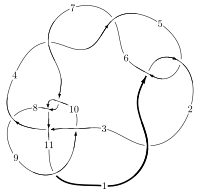
\includegraphics[width=112pt]{../../../GIT/diagram.site/Diagrams/png/416_11a_167.png}\\
\ \ \ A knot diagram\footnotemark}&
\allowdisplaybreaks
\textbf{Linearized knot diagam} \\
\cline{2-2}
 &
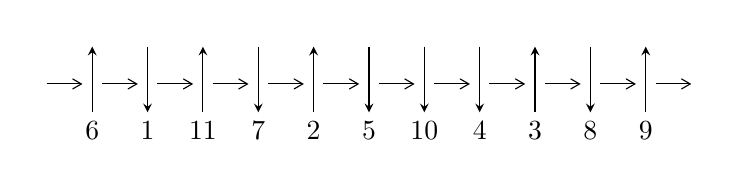
\begin{tikzpicture}[x=20pt, y=17pt]
	% nodes
	\node (C0) at (0, 0) {};
	\node (C1) at (1, 0) {};
	\node (C1U) at (1, +1) {};
	\node (C1D) at (1, -1) {6};

	\node (C2) at (2, 0) {};
	\node (C2U) at (2, +1) {};
	\node (C2D) at (2, -1) {1};

	\node (C3) at (3, 0) {};
	\node (C3U) at (3, +1) {};
	\node (C3D) at (3, -1) {11};

	\node (C4) at (4, 0) {};
	\node (C4U) at (4, +1) {};
	\node (C4D) at (4, -1) {7};

	\node (C5) at (5, 0) {};
	\node (C5U) at (5, +1) {};
	\node (C5D) at (5, -1) {2};

	\node (C6) at (6, 0) {};
	\node (C6U) at (6, +1) {};
	\node (C6D) at (6, -1) {5};

	\node (C7) at (7, 0) {};
	\node (C7U) at (7, +1) {};
	\node (C7D) at (7, -1) {10};

	\node (C8) at (8, 0) {};
	\node (C8U) at (8, +1) {};
	\node (C8D) at (8, -1) {4};

	\node (C9) at (9, 0) {};
	\node (C9U) at (9, +1) {};
	\node (C9D) at (9, -1) {3};

	\node (C10) at (10, 0) {};
	\node (C10U) at (10, +1) {};
	\node (C10D) at (10, -1) {8};

	\node (C11) at (11, 0) {};
	\node (C11U) at (11, +1) {};
	\node (C11D) at (11, -1) {9};
	\node (C12) at (12, 0) {};

	% arrows
	\draw[->,>={angle 60}]
	(C0) edge (C1) (C1) edge (C2) (C2) edge (C3) (C3) edge (C4) (C4) edge (C5) (C5) edge (C6) (C6) edge (C7) (C7) edge (C8) (C8) edge (C9) (C9) edge (C10) (C10) edge (C11) (C11) edge (C12) ;	\draw[->,>=stealth]
	(C1D) edge (C1U) (C2U) edge (C2D) (C3D) edge (C3U) (C4U) edge (C4D) (C5D) edge (C5U) (C6U) edge (C6D) (C7U) edge (C7D) (C8U) edge (C8D) (C9D) edge (C9U) (C10U) edge (C10D) (C11D) edge (C11U) ;
	\end{tikzpicture} \\
\hhline{~~} \\& 
\textbf{Solving Sequence} \\ \cline{2-2} 
 &
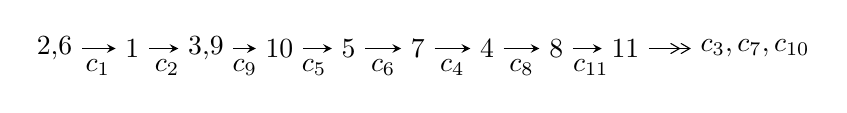
\begin{tikzpicture}[x=25pt, y=7pt]
	% node
	\node (A0) at (-1/8, 0) {2,6};
	\node (A1) at (1, 0) {1};
	\node (A2) at (33/16, 0) {3,9};
	\node (A3) at (25/8, 0) {10};
	\node (A4) at (33/8, 0) {5};
	\node (A5) at (41/8, 0) {7};
	\node (A6) at (49/8, 0) {4};
	\node (A7) at (57/8, 0) {8};
	\node (A8) at (65/8, 0) {11};
	\node (C1) at (1/2, -1) {$c_{1}$};
	\node (C2) at (3/2, -1) {$c_{2}$};
	\node (C3) at (21/8, -1) {$c_{9}$};
	\node (C4) at (29/8, -1) {$c_{5}$};
	\node (C5) at (37/8, -1) {$c_{6}$};
	\node (C6) at (45/8, -1) {$c_{4}$};
	\node (C7) at (53/8, -1) {$c_{8}$};
	\node (C8) at (61/8, -1) {$c_{11}$};
	\node (A9) at (10, 0) {$c_{3},c_{7},c_{10}$};

	% edge
	\draw[->,>=stealth]	
	(A0) edge (A1) (A1) edge (A2) (A2) edge (A3) (A3) edge (A4) (A4) edge (A5) (A5) edge (A6) (A6) edge (A7) (A7) edge (A8) ;
	\draw[->>,>={angle 60}]	
	(A8) edge (A9);
\end{tikzpicture} \\ 

\end{tabular} \\

\footnotetext{
The image of knot diagram is generated by the software ``\textbf{Draw programme}" developed by Andrew Bartholomew(\url{http://www.layer8.co.uk/maths/draw/index.htm\#Running-draw}), where we modified some parts for our purpose(\url{https://github.com/CATsTAILs/LinksPainter}).
}\phantom \\ \newline 
\centering \textbf{Ideals for irreducible components\footnotemark of $X_{\text{par}}$} 
 
\begin{align*}
I^u_{1}&=\langle 
-9.20331\times10^{18} u^{57}-1.37199\times10^{19} u^{56}+\cdots+3.39537\times10^{18} b-4.21028\times10^{18},\\
\phantom{I^u_{1}}&\phantom{= \langle  }7.03039\times10^{18} u^{57}+1.85492\times10^{19} u^{56}+\cdots+3.39537\times10^{18} a+2.49612\times10^{19},\;u^{58}+2 u^{57}+\cdots- u+1\rangle \\
I^u_{2}&=\langle 
b- u,\;a+u+1,\;u^2+u+1\rangle \\
\\
\end{align*}
\raggedright * 2 irreducible components of $\dim_{\mathbb{C}}=0$, with total 60 representations.\\
\footnotetext{All coefficients of polynomials are rational numbers. But the coefficients are sometimes approximated in decimal forms when there is not enough margin.}
\newpage
\renewcommand{\arraystretch}{1}
\centering \section*{I. $I^u_{1}= \langle -9.20\times10^{18} u^{57}-1.37\times10^{19} u^{56}+\cdots+3.40\times10^{18} b-4.21\times10^{18},\;7.03\times10^{18} u^{57}+1.85\times10^{19} u^{56}+\cdots+3.40\times10^{18} a+2.50\times10^{19},\;u^{58}+2 u^{57}+\cdots- u+1 \rangle$}
\flushleft \textbf{(i) Arc colorings}\\
\begin{tabular}{m{7pt} m{180pt} m{7pt} m{180pt} }
\flushright $a_{2}=$&$\begin{pmatrix}1\\0\end{pmatrix}$ \\
\flushright $a_{6}=$&$\begin{pmatrix}0\\u\end{pmatrix}$ \\
\flushright $a_{1}=$&$\begin{pmatrix}1\\u^2\end{pmatrix}$ \\
\flushright $a_{3}=$&$\begin{pmatrix}u^2+1\\u^4\end{pmatrix}$ \\
\flushright $a_{9}=$&$\begin{pmatrix}-2.07058 u^{57}-5.46309 u^{56}+\cdots+8.71905 u-7.35155\\2.71055 u^{57}+4.04078 u^{56}+\cdots+2.87153 u+1.24001\end{pmatrix}$ \\
\flushright $a_{10}=$&$\begin{pmatrix}0.0678518 u^{57}-1.33180 u^{56}+\cdots+7.13402 u-4.56590\\2.17215 u^{57}+3.03451 u^{56}+\cdots+4.72602 u+0.0399380\end{pmatrix}$ \\
\flushright $a_{5}=$&$\begin{pmatrix}- u\\u\end{pmatrix}$ \\
\flushright $a_{7}=$&$\begin{pmatrix}- u^3\\u^3+u\end{pmatrix}$ \\
\flushright $a_{4}=$&$\begin{pmatrix}- u^5- u\\u^5+u^3+u\end{pmatrix}$ \\
\flushright $a_{8}=$&$\begin{pmatrix}-0.236838 u^{57}-1.43795 u^{56}+\cdots+5.04652 u-4.51898\\2.07684 u^{57}+2.44455 u^{56}+\cdots+6.07889 u-0.359956\end{pmatrix}$ \\
\flushright $a_{11}=$&$\begin{pmatrix}-1.42519 u^{57}-1.02253 u^{56}+\cdots-3.40758 u-0.311267\\0.425182 u^{57}-1.40266 u^{56}+\cdots+2.31128 u-1.00001\end{pmatrix}$\\ \flushright $a_{11}=$&$\begin{pmatrix}-1.42519 u^{57}-1.02253 u^{56}+\cdots-3.40758 u-0.311267\\0.425182 u^{57}-1.40266 u^{56}+\cdots+2.31128 u-1.00001\end{pmatrix}$\\&\end{tabular}
\flushleft \textbf{(ii) Obstruction class $= -1$}\\~\\
\flushleft \textbf{(iii) Cusp Shapes $= -\frac{14190392272677106611}{3395365732110338209} u^{57}-\frac{62198624286930003489}{3395365732110338209} u^{56}+\cdots+\frac{132938789220611994229}{3395365732110338209} u-\frac{85221440426712296632}{3395365732110338209}$}\\~\\
\newpage\renewcommand{\arraystretch}{1}
\flushleft \textbf{(iv) u-Polynomials at the component}\newline \\
\begin{tabular}{m{50pt}|m{274pt}}
Crossings & \hspace{64pt}u-Polynomials at each crossing \\
\hline $$\begin{aligned}c_{1},c_{5}\end{aligned}$$&$\begin{aligned}
&u^{58}-2 u^{57}+\cdots+u+1
\end{aligned}$\\
\hline $$\begin{aligned}c_{2},c_{4},c_{6}\end{aligned}$$&$\begin{aligned}
&u^{58}+14 u^{57}+\cdots+5 u+1
\end{aligned}$\\
\hline $$\begin{aligned}c_{3}\end{aligned}$$&$\begin{aligned}
&u^{58}+4 u^{57}+\cdots+u+1
\end{aligned}$\\
\hline $$\begin{aligned}c_{7},c_{10}\end{aligned}$$&$\begin{aligned}
&u^{58}-3 u^{57}+\cdots-10 u+1
\end{aligned}$\\
\hline $$\begin{aligned}c_{8}\end{aligned}$$&$\begin{aligned}
&u^{58}-4 u^{57}+\cdots-21 u+1
\end{aligned}$\\
\hline $$\begin{aligned}c_{9}\end{aligned}$$&$\begin{aligned}
&u^{58}-2 u^{57}+\cdots+403 u+77
\end{aligned}$\\
\hline $$\begin{aligned}c_{11}\end{aligned}$$&$\begin{aligned}
&u^{58}+9 u^{57}+\cdots+12 u+4
\end{aligned}$\\
\hline
\end{tabular}\\~\\
\newpage\renewcommand{\arraystretch}{1}
\flushleft \textbf{(v) Riley Polynomials at the component}\newline \\
\begin{tabular}{m{50pt}|m{274pt}}
Crossings & \hspace{64pt}Riley Polynomials at each crossing \\
\hline $$\begin{aligned}c_{1},c_{5}\end{aligned}$$&$\begin{aligned}
&y^{58}+14 y^{57}+\cdots+5 y+1
\end{aligned}$\\
\hline $$\begin{aligned}c_{2},c_{4},c_{6}\end{aligned}$$&$\begin{aligned}
&y^{58}+62 y^{57}+\cdots+53 y+1
\end{aligned}$\\
\hline $$\begin{aligned}c_{3}\end{aligned}$$&$\begin{aligned}
&y^{58}+10 y^{57}+\cdots+5 y+1
\end{aligned}$\\
\hline $$\begin{aligned}c_{7},c_{10}\end{aligned}$$&$\begin{aligned}
&y^{58}-33 y^{57}+\cdots+122 y+1
\end{aligned}$\\
\hline $$\begin{aligned}c_{8}\end{aligned}$$&$\begin{aligned}
&y^{58}-46 y^{57}+\cdots+117 y+1
\end{aligned}$\\
\hline $$\begin{aligned}c_{9}\end{aligned}$$&$\begin{aligned}
&y^{58}-58 y^{57}+\cdots-89259 y+5929
\end{aligned}$\\
\hline $$\begin{aligned}c_{11}\end{aligned}$$&$\begin{aligned}
&y^{58}-15 y^{57}+\cdots-168 y+16
\end{aligned}$\\
\hline
\end{tabular}\\~\\
\newpage\flushleft \textbf{(vi) Complex Volumes and Cusp Shapes}
$$\begin{array}{c|c|c}  
\text{Solutions to }I^u_{1}& \I (\text{vol} + \sqrt{-1}CS) & \text{Cusp shape}\\
 \hline 
\begin{aligned}
u &= \phantom{-}0.440912 + 0.897881 I \\
a &= \phantom{-}1.28479 - 1.51068 I \\
b &= -0.655511 + 0.976043 I\end{aligned}
 & \phantom{-}0.81208 + 5.75126 I & \phantom{-0.000000 } 0. - 9.28589 I \\ \hline\begin{aligned}
u &= \phantom{-}0.440912 - 0.897881 I \\
a &= \phantom{-}1.28479 + 1.51068 I \\
b &= -0.655511 - 0.976043 I\end{aligned}
 & \phantom{-}0.81208 - 5.75126 I & \phantom{-0.000000 -}0. + 9.28589 I \\ \hline\begin{aligned}
u &= \phantom{-}0.051144 + 1.040470 I \\
a &= \phantom{-}0.694306 - 0.600130 I \\
b &= \phantom{-}0.0941538 - 0.0407924 I\end{aligned}
 & -5.22394 - 4.97791 I & -7.03726 + 5.31540 I \\ \hline\begin{aligned}
u &= \phantom{-}0.051144 - 1.040470 I \\
a &= \phantom{-}0.694306 + 0.600130 I \\
b &= \phantom{-}0.0941538 + 0.0407924 I\end{aligned}
 & -5.22394 + 4.97791 I & -7.03726 - 5.31540 I \\ \hline\begin{aligned}
u &= \phantom{-}0.332519 + 0.864557 I \\
a &= \phantom{-}1.019630 + 0.147782 I \\
b &= \phantom{-}0.137567 - 0.696892 I\end{aligned}
 & -3.63287 + 3.82995 I & -8.64205 - 8.99135 I \\ \hline\begin{aligned}
u &= \phantom{-}0.332519 - 0.864557 I \\
a &= \phantom{-}1.019630 - 0.147782 I \\
b &= \phantom{-}0.137567 + 0.696892 I\end{aligned}
 & -3.63287 - 3.82995 I & -8.64205 + 8.99135 I \\ \hline\begin{aligned}
u &= -0.336157 + 1.024860 I \\
a &= -0.225338 + 0.792429 I \\
b &= \phantom{-}0.112078 - 0.426502 I\end{aligned}
 & -1.05261 - 3.13615 I & \phantom{-0.000000 -}0. + 8.50381 I \\ \hline\begin{aligned}
u &= -0.336157 - 1.024860 I \\
a &= -0.225338 - 0.792429 I \\
b &= \phantom{-}0.112078 + 0.426502 I\end{aligned}
 & -1.05261 + 3.13615 I & \phantom{-0.000000 } 0. - 8.50381 I \\ \hline\begin{aligned}
u &= \phantom{-}0.434758 + 1.011700 I \\
a &= -1.05107 + 1.46627 I \\
b &= \phantom{-}0.635292 - 1.236510 I\end{aligned}
 & -2.95190 + 11.16430 I & \phantom{-0.000000 } 0. - 9.61832 I \\ \hline\begin{aligned}
u &= \phantom{-}0.434758 - 1.011700 I \\
a &= -1.05107 - 1.46627 I \\
b &= \phantom{-}0.635292 + 1.236510 I\end{aligned}
 & -2.95190 - 11.16430 I & \phantom{-0.000000 -}0. + 9.61832 I\\
 \hline 
 \end{array}$$\newpage$$\begin{array}{c|c|c}  
\text{Solutions to }I^u_{1}& \I (\text{vol} + \sqrt{-1}CS) & \text{Cusp shape}\\
 \hline 
\begin{aligned}
u &= -0.769063 + 0.455452 I \\
a &= -0.930791 + 0.294716 I \\
b &= \phantom{-}0.667321 + 0.337766 I\end{aligned}
 & \phantom{-}0.20150 - 3.82733 I & \phantom{-}2.45119 + 7.09206 I \\ \hline\begin{aligned}
u &= -0.769063 - 0.455452 I \\
a &= -0.930791 - 0.294716 I \\
b &= \phantom{-}0.667321 - 0.337766 I\end{aligned}
 & \phantom{-}0.20150 + 3.82733 I & \phantom{-}2.45119 - 7.09206 I \\ \hline\begin{aligned}
u &= -0.440330 + 0.759700 I \\
a &= -1.066630 - 0.436456 I \\
b &= \phantom{-}0.384922 + 0.669695 I\end{aligned}
 & \phantom{-}0.01176 - 1.74270 I & \phantom{-}0.45658 + 3.63727 I \\ \hline\begin{aligned}
u &= -0.440330 - 0.759700 I \\
a &= -1.066630 + 0.436456 I \\
b &= \phantom{-}0.384922 - 0.669695 I\end{aligned}
 & \phantom{-}0.01176 + 1.74270 I & \phantom{-}0.45658 - 3.63727 I \\ \hline\begin{aligned}
u &= \phantom{-}0.225458 + 0.825902 I \\
a &= -1.06368 + 2.01364 I \\
b &= \phantom{-}1.09293 - 1.05099 I\end{aligned}
 & -4.22808 + 0.48675 I & -11.22027 - 2.03951 I \\ \hline\begin{aligned}
u &= \phantom{-}0.225458 - 0.825902 I \\
a &= -1.06368 - 2.01364 I \\
b &= \phantom{-}1.09293 + 1.05099 I\end{aligned}
 & -4.22808 - 0.48675 I & -11.22027 + 2.03951 I \\ \hline\begin{aligned}
u &= -0.340458 + 0.770916 I \\
a &= \phantom{-}2.47350 - 3.28718 I \\
b &= -3.16149 + 0.03944 I\end{aligned}
 & -1.98107 - 1.64703 I & \phantom{-}6.1662 - 29.1207 I \\ \hline\begin{aligned}
u &= -0.340458 - 0.770916 I \\
a &= \phantom{-}2.47350 + 3.28718 I \\
b &= -3.16149 - 0.03944 I\end{aligned}
 & -1.98107 + 1.64703 I & \phantom{-}6.1662 + 29.1207 I \\ \hline\begin{aligned}
u &= -0.568190 + 1.020440 I \\
a &= \phantom{-}0.267371 - 0.661740 I \\
b &= -0.379130 + 0.546655 I\end{aligned}
 & -1.55389 - 1.10217 I & \phantom{-0.000000 } 0 \\ \hline\begin{aligned}
u &= -0.568190 - 1.020440 I \\
a &= \phantom{-}0.267371 + 0.661740 I \\
b &= -0.379130 - 0.546655 I\end{aligned}
 & -1.55389 + 1.10217 I & \phantom{-0.000000 } 0\\
 \hline 
 \end{array}$$\newpage$$\begin{array}{c|c|c}  
\text{Solutions to }I^u_{1}& \I (\text{vol} + \sqrt{-1}CS) & \text{Cusp shape}\\
 \hline 
\begin{aligned}
u &= \phantom{-}0.741876 + 0.285613 I \\
a &= -1.143890 + 0.651964 I \\
b &= \phantom{-}0.222922 - 0.926797 I\end{aligned}
 & -0.59272 - 6.92978 I & \phantom{-}1.28521 + 5.28654 I \\ \hline\begin{aligned}
u &= \phantom{-}0.741876 - 0.285613 I \\
a &= -1.143890 - 0.651964 I \\
b &= \phantom{-}0.222922 + 0.926797 I\end{aligned}
 & -0.59272 + 6.92978 I & \phantom{-}1.28521 - 5.28654 I \\ \hline\begin{aligned}
u &= -0.843359 + 0.871287 I \\
a &= -1.58053 + 0.99032 I \\
b &= \phantom{-}2.04212 + 0.61200 I\end{aligned}
 & \phantom{-}3.51042 + 0.65934 I & \phantom{-0.000000 } 0 \\ \hline\begin{aligned}
u &= -0.843359 - 0.871287 I \\
a &= -1.58053 - 0.99032 I \\
b &= \phantom{-}2.04212 - 0.61200 I\end{aligned}
 & \phantom{-}3.51042 - 0.65934 I & \phantom{-0.000000 } 0 \\ \hline\begin{aligned}
u &= \phantom{-}0.895121 + 0.818579 I \\
a &= \phantom{-}0.892761 - 0.255381 I \\
b &= -0.50150 + 1.65644 I\end{aligned}
 & \phantom{-}7.18623 - 1.43763 I & \phantom{-0.000000 } 0 \\ \hline\begin{aligned}
u &= \phantom{-}0.895121 - 0.818579 I \\
a &= \phantom{-}0.892761 + 0.255381 I \\
b &= -0.50150 - 1.65644 I\end{aligned}
 & \phantom{-}7.18623 + 1.43763 I & \phantom{-0.000000 } 0 \\ \hline\begin{aligned}
u &= -0.817614 + 0.900250 I \\
a &= -2.55651 - 1.15874 I \\
b &= \phantom{-}0.38714 + 3.85396 I\end{aligned}
 & \phantom{-}1.70109 - 3.05742 I & \phantom{-0.000000 } 0 \\ \hline\begin{aligned}
u &= -0.817614 - 0.900250 I \\
a &= -2.55651 + 1.15874 I \\
b &= \phantom{-}0.38714 - 3.85396 I\end{aligned}
 & \phantom{-}1.70109 + 3.05742 I & \phantom{-0.000000 } 0 \\ \hline\begin{aligned}
u &= -0.010811 + 0.780206 I \\
a &= -1.13083 + 1.06637 I \\
b &= \phantom{-}0.336641 + 0.147588 I\end{aligned}
 & -1.43717 - 1.52858 I & -5.32481 + 4.46151 I \\ \hline\begin{aligned}
u &= -0.010811 - 0.780206 I \\
a &= -1.13083 - 1.06637 I \\
b &= \phantom{-}0.336641 - 0.147588 I\end{aligned}
 & -1.43717 + 1.52858 I & -5.32481 - 4.46151 I\\
 \hline 
 \end{array}$$\newpage$$\begin{array}{c|c|c}  
\text{Solutions to }I^u_{1}& \I (\text{vol} + \sqrt{-1}CS) & \text{Cusp shape}\\
 \hline 
\begin{aligned}
u &= \phantom{-}0.848099 + 0.894531 I \\
a &= \phantom{-}1.07319 - 1.36400 I \\
b &= \phantom{-}1.65226 + 1.13672 I\end{aligned}
 & \phantom{-}5.05665 + 2.36415 I & \phantom{-0.000000 } 0 \\ \hline\begin{aligned}
u &= \phantom{-}0.848099 - 0.894531 I \\
a &= \phantom{-}1.07319 + 1.36400 I \\
b &= \phantom{-}1.65226 - 1.13672 I\end{aligned}
 & \phantom{-}5.05665 - 2.36415 I & \phantom{-0.000000 } 0 \\ \hline\begin{aligned}
u &= -0.910971 + 0.834834 I \\
a &= -1.39520 - 0.83245 I \\
b &= -0.16453 + 2.92280 I\end{aligned}
 & \phantom{-}5.95099 + 9.03935 I & \phantom{-0.000000 } 0 \\ \hline\begin{aligned}
u &= -0.910971 - 0.834834 I \\
a &= -1.39520 + 0.83245 I \\
b &= -0.16453 - 2.92280 I\end{aligned}
 & \phantom{-}5.95099 - 9.03935 I & \phantom{-0.000000 } 0 \\ \hline\begin{aligned}
u &= -0.885584 + 0.866640 I \\
a &= \phantom{-}1.50974 + 1.18822 I \\
b &= \phantom{-}0.37841 - 3.18031 I\end{aligned}
 & \phantom{-}9.19750 + 2.53947 I & \phantom{-0.000000 } 0 \\ \hline\begin{aligned}
u &= -0.885584 - 0.866640 I \\
a &= \phantom{-}1.50974 - 1.18822 I \\
b &= \phantom{-}0.37841 + 3.18031 I\end{aligned}
 & \phantom{-}9.19750 - 2.53947 I & \phantom{-0.000000 } 0 \\ \hline\begin{aligned}
u &= -0.823065 + 0.934173 I \\
a &= \phantom{-}0.54799 - 1.61489 I \\
b &= -1.96451 + 1.14977 I\end{aligned}
 & \phantom{-}3.31523 - 6.86856 I & \phantom{-0.000000 } 0 \\ \hline\begin{aligned}
u &= -0.823065 - 0.934173 I \\
a &= \phantom{-}0.54799 + 1.61489 I \\
b &= -1.96451 - 1.14977 I\end{aligned}
 & \phantom{-}3.31523 + 6.86856 I & \phantom{-0.000000 } 0 \\ \hline\begin{aligned}
u &= \phantom{-}0.838722 + 0.920465 I \\
a &= \phantom{-}0.561004 + 0.957597 I \\
b &= -1.93336 + 1.29288 I\end{aligned}
 & \phantom{-}4.97538 + 3.90988 I & \phantom{-0.000000 } 0 \\ \hline\begin{aligned}
u &= \phantom{-}0.838722 - 0.920465 I \\
a &= \phantom{-}0.561004 - 0.957597 I \\
b &= -1.93336 - 1.29288 I\end{aligned}
 & \phantom{-}4.97538 - 3.90988 I & \phantom{-0.000000 } 0\\
 \hline 
 \end{array}$$\newpage$$\begin{array}{c|c|c}  
\text{Solutions to }I^u_{1}& \I (\text{vol} + \sqrt{-1}CS) & \text{Cusp shape}\\
 \hline 
\begin{aligned}
u &= \phantom{-}0.897894 + 0.891847 I \\
a &= -1.155740 + 0.290111 I \\
b &= \phantom{-}0.41707 - 1.99877 I\end{aligned}
 & \phantom{-}8.46147 + 2.78521 I & \phantom{-0.000000 } 0 \\ \hline\begin{aligned}
u &= \phantom{-}0.897894 - 0.891847 I \\
a &= -1.155740 - 0.290111 I \\
b &= \phantom{-}0.41707 + 1.99877 I\end{aligned}
 & \phantom{-}8.46147 - 2.78521 I & \phantom{-0.000000 } 0 \\ \hline\begin{aligned}
u &= \phantom{-}0.590155 + 0.416456 I \\
a &= \phantom{-}0.964716 - 0.975316 I \\
b &= -0.411626 + 0.943907 I\end{aligned}
 & \phantom{-}2.32246 - 1.88820 I & \phantom{-}5.25997 + 2.06026 I \\ \hline\begin{aligned}
u &= \phantom{-}0.590155 - 0.416456 I \\
a &= \phantom{-}0.964716 + 0.975316 I \\
b &= -0.411626 - 0.943907 I\end{aligned}
 & \phantom{-}2.32246 + 1.88820 I & \phantom{-}5.25997 - 2.06026 I \\ \hline\begin{aligned}
u &= -0.845331 + 0.960143 I \\
a &= \phantom{-}2.46844 + 0.68770 I \\
b &= -0.88375 - 3.17281 I\end{aligned}
 & \phantom{-}8.90043 - 8.94791 I & \phantom{-0.000000 } 0 \\ \hline\begin{aligned}
u &= -0.845331 - 0.960143 I \\
a &= \phantom{-}2.46844 - 0.68770 I \\
b &= -0.88375 + 3.17281 I\end{aligned}
 & \phantom{-}8.90043 + 8.94791 I & \phantom{-0.000000 } 0 \\ \hline\begin{aligned}
u &= \phantom{-}0.867514 + 0.951168 I \\
a &= -1.31254 + 0.69248 I \\
b &= -0.09282 - 2.05203 I\end{aligned}
 & \phantom{-}8.26855 + 3.73272 I & \phantom{-0.000000 } 0 \\ \hline\begin{aligned}
u &= \phantom{-}0.867514 - 0.951168 I \\
a &= -1.31254 - 0.69248 I \\
b &= -0.09282 + 2.05203 I\end{aligned}
 & \phantom{-}8.26855 - 3.73272 I & \phantom{-0.000000 } 0 \\ \hline\begin{aligned}
u &= \phantom{-}0.823019 + 0.992908 I \\
a &= \phantom{-}1.17187 - 0.87639 I \\
b &= \phantom{-}0.13038 + 1.73093 I\end{aligned}
 & \phantom{-}6.63609 + 7.79931 I & \phantom{-0.000000 } 0 \\ \hline\begin{aligned}
u &= \phantom{-}0.823019 - 0.992908 I \\
a &= \phantom{-}1.17187 + 0.87639 I \\
b &= \phantom{-}0.13038 - 1.73093 I\end{aligned}
 & \phantom{-}6.63609 - 7.79931 I & \phantom{-0.000000 } 0\\
 \hline 
 \end{array}$$\newpage$$\begin{array}{c|c|c}  
\text{Solutions to }I^u_{1}& \I (\text{vol} + \sqrt{-1}CS) & \text{Cusp shape}\\
 \hline 
\begin{aligned}
u &= -0.839643 + 0.992004 I \\
a &= -2.25810 - 0.80518 I \\
b &= \phantom{-}0.57202 + 3.02731 I\end{aligned}
 & \phantom{-}5.4499 - 15.5032 I & \phantom{-0.000000 } 0 \\ \hline\begin{aligned}
u &= -0.839643 - 0.992004 I \\
a &= -2.25810 + 0.80518 I \\
b &= \phantom{-}0.57202 - 3.02731 I\end{aligned}
 & \phantom{-}5.4499 + 15.5032 I & \phantom{-0.000000 } 0 \\ \hline\begin{aligned}
u &= -0.310122 + 0.582175 I \\
a &= -1.49433 + 2.38673 I \\
b &= \phantom{-}1.265490 + 0.474592 I\end{aligned}
 & -1.39991 - 1.11754 I & -8.74885 + 3.65436 I \\ \hline\begin{aligned}
u &= -0.310122 - 0.582175 I \\
a &= -1.49433 - 2.38673 I \\
b &= \phantom{-}1.265490 - 0.474592 I\end{aligned}
 & -1.39991 + 1.11754 I & -8.74885 - 3.65436 I \\ \hline\begin{aligned}
u &= -0.587529 + 0.195087 I \\
a &= \phantom{-}0.575520 - 0.301118 I \\
b &= -0.685426 - 0.097381 I\end{aligned}
 & \phantom{-}1.59378 - 0.29446 I & \phantom{-}6.92249 - 0.09350 I \\ \hline\begin{aligned}
u &= -0.587529 - 0.195087 I \\
a &= \phantom{-}0.575520 + 0.301118 I \\
b &= -0.685426 + 0.097381 I\end{aligned}
 & \phantom{-}1.59378 + 0.29446 I & \phantom{-}6.92249 + 0.09350 I \\ \hline\begin{aligned}
u &= \phantom{-}0.341034 + 0.197878 I \\
a &= -2.63966 + 0.02210 I \\
b &= \phantom{-}0.304941 + 0.449084 I\end{aligned}
 & -1.92464 - 1.08312 I & -1.72371 + 1.84781 I \\ \hline\begin{aligned}
u &= \phantom{-}0.341034 - 0.197878 I \\
a &= -2.63966 - 0.02210 I \\
b &= \phantom{-}0.304941 - 0.449084 I\end{aligned}
 & -1.92464 + 1.08312 I & -1.72371 - 1.84781 I\\
 \hline 
 \end{array}$$\newpage\newpage\renewcommand{\arraystretch}{1}
\centering \section*{II. $I^u_{2}= \langle b- u,\;a+u+1,\;u^2+u+1 \rangle$}
\flushleft \textbf{(i) Arc colorings}\\
\begin{tabular}{m{7pt} m{180pt} m{7pt} m{180pt} }
\flushright $a_{2}=$&$\begin{pmatrix}1\\0\end{pmatrix}$ \\
\flushright $a_{6}=$&$\begin{pmatrix}0\\u\end{pmatrix}$ \\
\flushright $a_{1}=$&$\begin{pmatrix}1\\- u-1\end{pmatrix}$ \\
\flushright $a_{3}=$&$\begin{pmatrix}- u\\u\end{pmatrix}$ \\
\flushright $a_{9}=$&$\begin{pmatrix}- u-1\\u\end{pmatrix}$ \\
\flushright $a_{10}=$&$\begin{pmatrix}0\\-1\end{pmatrix}$ \\
\flushright $a_{5}=$&$\begin{pmatrix}- u\\u\end{pmatrix}$ \\
\flushright $a_{7}=$&$\begin{pmatrix}-1\\u+1\end{pmatrix}$ \\
\flushright $a_{4}=$&$\begin{pmatrix}1\\0\end{pmatrix}$ \\
\flushright $a_{8}=$&$\begin{pmatrix}-1\\u\end{pmatrix}$ \\
\flushright $a_{11}=$&$\begin{pmatrix}1\\- u-1\end{pmatrix}$\\ \flushright $a_{11}=$&$\begin{pmatrix}1\\- u-1\end{pmatrix}$\\&\end{tabular}
\flushleft \textbf{(ii) Obstruction class $= 1$}\\~\\
\flushleft \textbf{(iii) Cusp Shapes $= 4 u-1$}\\~\\
\newpage\renewcommand{\arraystretch}{1}
\flushleft \textbf{(iv) u-Polynomials at the component}\newline \\
\begin{tabular}{m{50pt}|m{274pt}}
Crossings & \hspace{64pt}u-Polynomials at each crossing \\
\hline $$\begin{aligned}c_{1},c_{2},c_{3}\\c_{6}\end{aligned}$$&$\begin{aligned}
&u^2+u+1
\end{aligned}$\\
\hline $$\begin{aligned}c_{4},c_{5},c_{8}\\c_{9}\end{aligned}$$&$\begin{aligned}
&u^2- u+1
\end{aligned}$\\
\hline $$\begin{aligned}c_{7}\end{aligned}$$&$\begin{aligned}
&(u-1)^2
\end{aligned}$\\
\hline $$\begin{aligned}c_{10}\end{aligned}$$&$\begin{aligned}
&(u+1)^2
\end{aligned}$\\
\hline $$\begin{aligned}c_{11}\end{aligned}$$&$\begin{aligned}
&u^2
\end{aligned}$\\
\hline
\end{tabular}\\~\\
\newpage\renewcommand{\arraystretch}{1}
\flushleft \textbf{(v) Riley Polynomials at the component}\newline \\
\begin{tabular}{m{50pt}|m{274pt}}
Crossings & \hspace{64pt}Riley Polynomials at each crossing \\
\hline $$\begin{aligned}c_{1},c_{2},c_{3}\\c_{4},c_{5},c_{6}\\c_{8},c_{9}\end{aligned}$$&$\begin{aligned}
&y^2+y+1
\end{aligned}$\\
\hline $$\begin{aligned}c_{7},c_{10}\end{aligned}$$&$\begin{aligned}
&(y-1)^2
\end{aligned}$\\
\hline $$\begin{aligned}c_{11}\end{aligned}$$&$\begin{aligned}
&y^2
\end{aligned}$\\
\hline
\end{tabular}\\~\\
\newpage\flushleft \textbf{(vi) Complex Volumes and Cusp Shapes}
$$\begin{array}{c|c|c}  
\text{Solutions to }I^u_{2}& \I (\text{vol} + \sqrt{-1}CS) & \text{Cusp shape}\\
 \hline 
\begin{aligned}
u &= -0.500000 + 0.866025 I \\
a &= -0.500000 - 0.866025 I \\
b &= -0.500000 + 0.866025 I\end{aligned}
 & -1.64493 - 2.02988 I & -3.00000 + 3.46410 I \\ \hline\begin{aligned}
u &= -0.500000 - 0.866025 I \\
a &= -0.500000 + 0.866025 I \\
b &= -0.500000 - 0.866025 I\end{aligned}
 & -1.64493 + 2.02988 I & -3.00000 - 3.46410 I\\
 \hline 
 \end{array}$$\newpage
\newpage\renewcommand{\arraystretch}{1}
\centering \section*{ III. u-Polynomials}
\begin{tabular}{m{50pt}|m{274pt}}
Crossings & \hspace{64pt}u-Polynomials at each crossing \\
\hline $$\begin{aligned}c_{1}\end{aligned}$$&$\begin{aligned}
&(u^2+u+1)(u^{58}-2 u^{57}+\cdots+u+1)
\end{aligned}$\\
\hline $$\begin{aligned}c_{2},c_{6}\end{aligned}$$&$\begin{aligned}
&(u^2+u+1)(u^{58}+14 u^{57}+\cdots+5 u+1)
\end{aligned}$\\
\hline $$\begin{aligned}c_{3}\end{aligned}$$&$\begin{aligned}
&(u^2+u+1)(u^{58}+4 u^{57}+\cdots+u+1)
\end{aligned}$\\
\hline $$\begin{aligned}c_{4}\end{aligned}$$&$\begin{aligned}
&(u^2- u+1)(u^{58}+14 u^{57}+\cdots+5 u+1)
\end{aligned}$\\
\hline $$\begin{aligned}c_{5}\end{aligned}$$&$\begin{aligned}
&(u^2- u+1)(u^{58}-2 u^{57}+\cdots+u+1)
\end{aligned}$\\
\hline $$\begin{aligned}c_{7}\end{aligned}$$&$\begin{aligned}
&((u-1)^2)(u^{58}-3 u^{57}+\cdots-10 u+1)
\end{aligned}$\\
\hline $$\begin{aligned}c_{8}\end{aligned}$$&$\begin{aligned}
&(u^2- u+1)(u^{58}-4 u^{57}+\cdots-21 u+1)
\end{aligned}$\\
\hline $$\begin{aligned}c_{9}\end{aligned}$$&$\begin{aligned}
&(u^2- u+1)(u^{58}-2 u^{57}+\cdots+403 u+77)
\end{aligned}$\\
\hline $$\begin{aligned}c_{10}\end{aligned}$$&$\begin{aligned}
&((u+1)^2)(u^{58}-3 u^{57}+\cdots-10 u+1)
\end{aligned}$\\
\hline $$\begin{aligned}c_{11}\end{aligned}$$&$\begin{aligned}
&u^2(u^{58}+9 u^{57}+\cdots+12 u+4)
\end{aligned}$\\
\hline
\end{tabular}\newpage\renewcommand{\arraystretch}{1}
\centering \section*{ IV. Riley Polynomials}
\begin{tabular}{m{50pt}|m{274pt}}
Crossings & \hspace{64pt}Riley Polynomials at each crossing \\
\hline $$\begin{aligned}c_{1},c_{5}\end{aligned}$$&$\begin{aligned}
&(y^2+y+1)(y^{58}+14 y^{57}+\cdots+5 y+1)
\end{aligned}$\\
\hline $$\begin{aligned}c_{2},c_{4},c_{6}\end{aligned}$$&$\begin{aligned}
&(y^2+y+1)(y^{58}+62 y^{57}+\cdots+53 y+1)
\end{aligned}$\\
\hline $$\begin{aligned}c_{3}\end{aligned}$$&$\begin{aligned}
&(y^2+y+1)(y^{58}+10 y^{57}+\cdots+5 y+1)
\end{aligned}$\\
\hline $$\begin{aligned}c_{7},c_{10}\end{aligned}$$&$\begin{aligned}
&((y-1)^2)(y^{58}-33 y^{57}+\cdots+122 y+1)
\end{aligned}$\\
\hline $$\begin{aligned}c_{8}\end{aligned}$$&$\begin{aligned}
&(y^2+y+1)(y^{58}-46 y^{57}+\cdots+117 y+1)
\end{aligned}$\\
\hline $$\begin{aligned}c_{9}\end{aligned}$$&$\begin{aligned}
&(y^2+y+1)(y^{58}-58 y^{57}+\cdots-89259 y+5929)
\end{aligned}$\\
\hline $$\begin{aligned}c_{11}\end{aligned}$$&$\begin{aligned}
&y^2(y^{58}-15 y^{57}+\cdots-168 y+16)
\end{aligned}$\\
\hline
\end{tabular}
\vskip 2pc
\end{document}